\documentclass{standalone}

\usepackage{tikz}

\usepackage{xcolor}
\definecolor{border}{gray}{0.66}
\definecolor{darktan}{rgb}{0.475,0.369,0.263}
\definecolor{tan}{rgb}{0.702,0.541,0.329}
\definecolor{darkred}{rgb}{0.51,0.102,0.059}
\definecolor{red}{rgb}{0.698,0.098,0.027}
\definecolor{darkblue}{rgb}{0.149,0.2,0.0235}
\definecolor{blue}{rgb}{0.18,0.247,0.318}

\newcommand{\drawblock}[3]{%
    \begin{scope}[shift={(2*#2,2*#3)}]
        \foreach \x/\y in {0/0,0/1,1/0,1/1}{
            \node[circle,draw=dark#1,fill=#1,minimum size=5ex] at (\x,\y) {};
        }
    \end{scope}
}

\begin{document}
    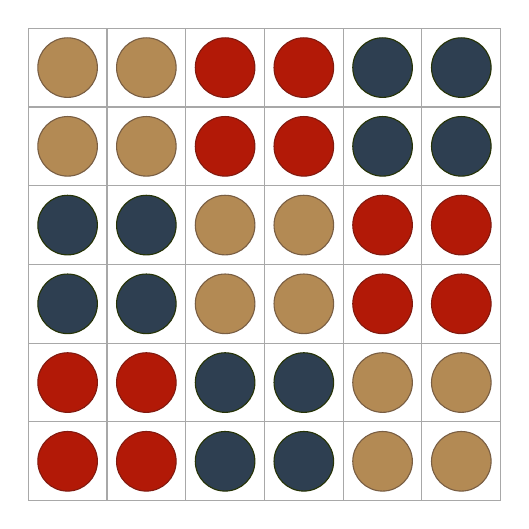
\begin{tikzpicture}
        \begin{scope}[shift={(-0.5,-0.5)}]
            \foreach \i in {0,...,6}{
                \draw[border] (\i,0) -- (\i,6);
                \draw[border] (0,\i) -- (6,\i);
            }
        \end{scope}
        
        \foreach \i/\j in {0/2,1/1,2/0}{%
            \drawblock{tan}{\i}{\j}
        }
        
        \foreach \i/\j in {0/0,1/2,2/1}{%
            \drawblock{red}{\i}{\j}
        }
    
        \foreach \i/\j in {0/1,1/0,2/2}{%
            \drawblock{blue}{\i}{\j}
        }
    \end{tikzpicture}
\end{document}